% This is "sig-alternate.tex" V2.1 April 2013
% This file should be compiled with V2.5 of "sig-alternate.cls" May 2012
%
% This example file demonstrates the use of the 'sig-alternate.cls'
% V2.5 LaTeX2e document class file. It is for those submitting
% articles to ACM Conference Proceedings WHO DO NOT WISH TO
% STRICTLY ADHERE TO THE SIGS (PUBS-BOARD-ENDORSED) STYLE.
% The 'sig-alternate.cls' file will produce a similar-looking,
% albeit, 'tighter' paper resulting in, invariably, fewer pages.
%
% ----------------------------------------------------------------------------------------------------------------
% This .tex file (and associated .cls V2.5) produces:
%       1) The Permission Statement
%       2) The Conference (location) Info information
%       3) The Copyright Line with ACM data
%       4) NO page numbers
%
% as against the acm_proc_article-sp.cls file which
% DOES NOT produce 1) thru' 3) above.
%
% Using 'sig-alternate.cls' you have control, however, from within
% the source .tex file, over both the CopyrightYear
% (defaulted to 200X) and the ACM Copyright Data
% (defaulted to X-XXXXX-XX-X/XX/XX).
% e.g.
% \CopyrightYear{2007} will cause 2007 to appear in the copyright line.
% \crdata{0-12345-67-8/90/12} will cause 0-12345-67-8/90/12 to appear in the copyright line.
%
% ---------------------------------------------------------------------------------------------------------------
% This .tex source is an example which *does* use
% the .bib file (from which the .bbl file % is produced).
% REMEMBER HOWEVER: After having produced the .bbl file,
% and prior to final submission, you *NEED* to 'insert'
% your .bbl file into your source .tex file so as to provide
% ONE 'self-contained' source file.
%
% ================= IF YOU HAVE QUESTIONS =======================
% Questions regarding the SIGS styles, SIGS policies and
% procedures, Conferences etc. should be sent to
% Adrienne Griscti (griscti@acm.org)
%
% Technical questions _only_ to
% Gerald Murray (murray@hq.acm.org)
% ===============================================================
%
% For tracking purposes - this is V2.0 - May 2012

\documentclass{sig-alternate-05-2015}
\usepackage{subfigure}
\usepackage{enumitem}
\usepackage[ruled,vlined,linesnumbered]{algorithm2e}
\usepackage{algorithm}
\usepackage{algorithmic}
\usepackage{bm}

\usepackage{array}
\newcolumntype{L}[1]{>{\raggedright\let\newline\\\arraybackslash\hspace{0pt}}m{#1}}
\newcolumntype{C}[1]{>{\centering\let\newline\\\arraybackslash\hspace{0pt}}m{#1}}
\newcolumntype{R}[1]{>{\raggedleft\let\newline\\\arraybackslash\hspace{0pt}}m{#1}}

%\makeatletter
%\def\@copyrightspace{\relax}
%\makeatother


\begin{document}

% Copyright
\setcopyright{acmcopyright}
%\setcopyright{acmlicensed}
%\setcopyright{rightsretained}
%\setcopyright{usgov}
%\setcopyright{usgovmixed}
%\setcopyright{cagov}
%\setcopyright{cagovmixed}


% DOI
%\doi{10.475/123_4}
\doi{**.***/***}

% ISBN
%\isbn{123-4567-24-567/08/06}
\isbn{***-****-**-***/**/**}

%Conference
%\conferenceinfo{PLDI '13}{June 16--19, 2013, Seattle, WA, USA}

%\acmPrice{\$15.00}

%
% --- Author Metadata here ---
%\conferenceinfo{WOODSTOCK}{'97 El Paso, Texas USA}
%\CopyrightYear{2007} % Allows default copyright year (20XX) to be over-ridden - IF NEED BE.
%\crdata{0-12345-67-8/90/01}  % Allows default copyright data (0-89791-88-6/97/05) to be over-ridden - IF NEED BE.
% --- End of Author Metadata ---

\title{Full History Info Enhanced Normal States Training for High Accuracy Event Detection}

%
% You need the command \numberofauthors to handle the 'placement
% and alignment' of the authors beneath the title.
%
% For aesthetic reasons, we recommend 'three authors at a time'
% i.e. three 'name/affiliation blocks' be placed beneath the title.
%
% NOTE: You are NOT restricted in how many 'rows' of
% "name/affiliations" may appear. We just ask that you restrict
% the number of 'columns' to three.
%
% Because of the available 'opening page real-estate'
% we ask you to refrain from putting more than six authors
% (two rows with three columns) beneath the article title.
% More than six makes the first-page appear very cluttered indeed.
%
% Use the \alignauthor commands to handle the names
% and affiliations for an 'aesthetic maximum' of six authors.
% Add names, affiliations, addresses for
% the seventh etc. author(s) as the argument for the
% \additionalauthors command.
% These 'additional authors' will be output/set for you
% without further effort on your part as the last section in
% the body of your article BEFORE References or any Appendices.

\begin{comment}
\numberofauthors{8} %  in this sample file, there are a *total*
% of EIGHT authors. SIX appear on the 'first-page' (for formatting
% reasons) and the remaining two appear in the \additionalauthors section.
%
\author{
% You can go ahead and credit any number of authors here,
% e.g. one 'row of three' or two rows (consisting of one row of three
% and a second row of one, two or three).
%
% The command \alignauthor (no curly braces needed) should
% precede each author name, affiliation/snail-mail address and
% e-mail address. Additionally, tag each line of
% affiliation/address with \affaddr, and tag the
% e-mail address with \email.
%
% 1st. author
\alignauthor
Ben Trovato\titlenote{Dr.~Trovato insisted his name be first.}\\
       \affaddr{Institute for Clarity in Documentation}\\
       \affaddr{1932 Wallamaloo Lane}\\
       \affaddr{Wallamaloo, New Zealand}\\
       \email{trovato@corporation.com}
% 2nd. author
\alignauthor
G.K.M. Tobin\titlenote{The secretary disavows
any knowledge of this author's actions.}\\
       \affaddr{Institute for Clarity in Documentation}\\
       \affaddr{P.O. Box 1212}\\
       \affaddr{Dublin, Ohio 43017-6221}\\
       \email{webmaster@marysville-ohio.com}
% 3rd. author
\alignauthor Lars Th{\o}rv{\"a}ld\titlenote{This author is the
one who did all the really hard work.}\\
       \affaddr{The Th{\o}rv{\"a}ld Group}\\
       \affaddr{1 Th{\o}rv{\"a}ld Circle}\\
       \affaddr{Hekla, Iceland}\\
       \email{larst@affiliation.org}
\and  % use '\and' if you need 'another row' of author names
% 4th. author
\alignauthor Lawrence P. Leipuner\\
       \affaddr{Brookhaven Laboratories}\\
       \affaddr{Brookhaven National Lab}\\
       \affaddr{P.O. Box 5000}\\
       \email{lleipuner@researchlabs.org}
% 5th. author
\alignauthor Sean Fogarty\\
       \affaddr{NASA Ames Research Center}\\
       \affaddr{Moffett Field}\\
       \affaddr{California 94035}\\
       \email{fogartys@amesres.org}
% 6th. author
\alignauthor Charles Palmer\\
       \affaddr{Palmer Research Laboratories}\\
       \affaddr{8600 Datapoint Drive}\\
       \affaddr{San Antonio, Texas 78229}\\
       \email{cpalmer@prl.com}
}
% There's nothing stopping you putting the seventh, eighth, etc.
% author on the opening page (as the 'third row') but we ask,
% for aesthetic reasons that you place these 'additional authors'
% in the \additional authors block, viz.
\additionalauthors{Additional authors: John Smith (The Th{\o}rv{\"a}ld Group,
email: {\texttt{jsmith@affiliation.org}}) and Julius P.~Kumquat
(The Kumquat Consortium, email: {\texttt{jpkumquat@consortium.net}}).}
\date{30 July 1999}
\end{comment}
% Just remember to make sure that the TOTAL number of authors
% is the number that will appear on the first page PLUS the
% number that will appear in the \additionalauthors section.

\maketitle
\begin{abstract}
In cyberspace, it is a very challenging task to detect events accurately due to its rapid changing nature.
In our study, we find out the key to improve the accuracy lies in training the normal states well, which describe what happened and help to identify what is happening in cyberspace.
Traditional methods underestimate the normal states due to the limited training data spanning over a few time windows.
To overcome this limitation, we propose \textsc{FullReader}, a high accuracy event detection system that trains normal states better by using Wikipedia, which can be treated as an approximation of full history information source. 
In \textsc{FullReader}, 1) normal states are trained as topical word frequencies; 2) historical topical word frequencies are extracted from Wikipedia pages, categories, and their Topic-PageRank-HITS scores; 3) topical word frequencies of targeted corpus are updated incrementally by Asymmetric-Prior-LDA, using the history information as prior; 4) events are detected by monitoring the change of topical word frequencies. 
Experiments on the benchmark Edinburgh twitter corpus validate the effectiveness of our proposed \textsc{FullReader}.
\end{abstract}


%
% The code below should be generated by the tool at
% http://dl.acm.org/ccs.cfm
% Please copy and paste the code instead of the example below. 
%
\begin{CCSXML}
<ccs2012>
 <concept>
  <concept_id>10010520.10010553.10010562</concept_id>
  <concept_desc>Computer systems organization~Embedded systems</concept_desc>
  <concept_significance>500</concept_significance>
 </concept>
 <concept>
  <concept_id>10010520.10010575.10010755</concept_id>
  <concept_desc>Computer systems organization~Redundancy</concept_desc>
  <concept_significance>300</concept_significance>
 </concept>
 <concept>
  <concept_id>10010520.10010553.10010554</concept_id>
  <concept_desc>Computer systems organization~Robotics</concept_desc>
  <concept_significance>100</concept_significance>
 </concept>
 <concept>
  <concept_id>10003033.10003083.10003095</concept_id>
  <concept_desc>Networks~Network reliability</concept_desc>
  <concept_significance>100</concept_significance>
 </concept>
</ccs2012>  
\end{CCSXML}

\ccsdesc{Mathematics of computing~Bayesian computation}
\ccsdesc{Mathematics of computing~Gibbs sampling}
\ccsdesc{Information systems ~ Data analytics}
\ccsdesc{Information systems ~Data stream mining}


%
% End generated code
%

%
%  Use this command to print the description
%
\printccsdesc

% We no longer use \terms command
%\terms{Theory}

\keywords{Full history info; normal states initialization and maintenance; event detection; text mining;}

\section{Introduction}
Improving the accuracy of event detection in cyberspace can benefit many tasks, but it's nontrivial due to the rapid changing nature of cyberspace.

In our study, we find out that the key to improve the accuracy of event detection lies in training the normal states of the focused media/site/domain. Based on training normal states accurately, event detection task can be treated as finding terms, articles, or topics which are different from the normal states. 

Our intuition is inspired from the news value theory\cite{galtung1965structure}\cite{caple2013delving}, which emphasizes the \textit{news unexpectedness} -- "the unpredictable or the rare is more newsworthy than the routine"\cite{bell1991language}, and "routine events are difficult to assimilate to the news, which favours the novel, the atypical and the unusual"\cite{montgomery2007discourse}.
Following this guideline, if the journalist knew the normal states, aka, the "routine things" of everyday better, he/she would tend to choose more unexpected news to report. 
We suppose that the ideal event detection system performs like a journalist who can find news from cyberspace with the knowledge of the normal states. 

To train the normal states, the methods of existing systems can be grouped into two categories: \textit{unsupervised normal states training} and \textit{classification based normal states training}, which is illustrated by Figure \ref{fig:modelDesc:a}.

In the first category, the methods treat the normal states as clustered articles\cite{Petrovic:2010uj}\cite{Wurzer:2015wq}, word frequencies\cite{Mathioudakis:2010fc}\cite{Weng:2011wz}, or topics\cite{Diao:2012wj}\cite{Yan:2015wm}. 
Taking the clustering of articles\cite{Petrovic:2010uj}\cite{Wurzer:2015wq} as an example, they model the occured events as clusters, and link the incoming article with an existing event cluster or assign it as the new detected event.
The decision is based on whether the dissimilarity between the incoming article and existing event clusters is over the user-specified threshold. 

And in the second category, the methods learn the normal states by given the knowledge of \textit{event trigger}\cite{Li2013JointEE}\cite{Nguyen2015EventDA} (usually a single verb or entity mentions). The normal states are trained by the labeled data appeared in a fixed time window.

Both categories of methods have achieved good performance on formal texts, but are hamppered by the diverse and rapid changing nature of cyberspace data (e.g., twitter\cite{Asur:2011tc} and reddit\cite{singer2014evolution}).
In the journalist metaphor of news value theory, they have the limited knowledge of normal states (aka "routine things") due to the limited history information used. 
More specifically, 


It's difficult to represent the 
the low threshold leads to , while the high threshold leads to 

They build the normal states in the evolving training window
%TODO
The second category, train the triggers\cite{Li2013JointEE}\cite{Nguyen2015EventDA}(\textit{But it has some problems here, these methods are used in event extraction, so what's the relationship between event extraction and event detection? and the fired example in \cite{Li2013JointEE}?}). 

They are hamppered by the rapid changing nature of cyberspace, e.g. twitter and reddit(\textit{find out the sentences to describe the rapid changing nature}). 

It is hard to handle all the cyberspace data by using limited computing resources. As a result, it have to make a trade off, only to process part of them, instead of using the whole data. 



In this paper, we demonstrate that the better normal states  are learned, the better event detection system can perform.

 and \textit{full history info enhanced normal states training}. 

\begin{figure*}[ht]
    \centering
    \subfigure[The first category methods\cite{Petrovic:2010uj}\cite{Wurzer:2015wq} utilize the history information appeared in an evolving training window; the second category\cite{Li2013JointEE}\cite{Nguyen2015EventDA} trains the normal states by the labeled data existed in a fixed time window. Our method intializes the normal states with full history info, and updates them incrementally. With normal states, systems detect events.]{
                \label{fig:modelDesc:a} %% label for first subfigure
                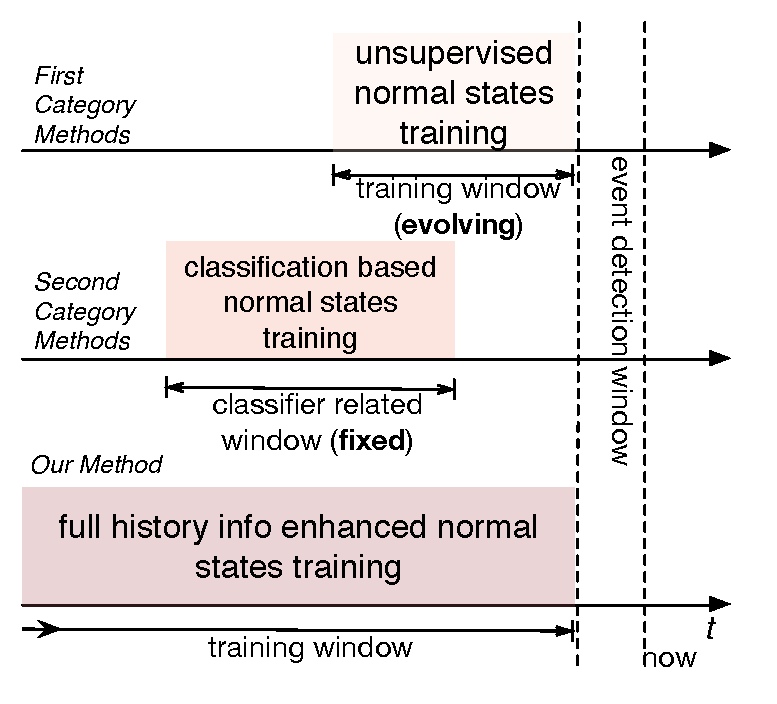
\includegraphics[height=7.4cm]{img/modelDescription.pdf}
        }
        \quad
        \quad
    \subfigure[\textsc{FullReader}'s process flow, taking \textbf{military} related events in cyberspace as an example. \textsc{FullReader} initializes the normal states as topical word frequencies from full history information about military, updates them further at the specific corpus day by day, and detects events finally.]{
                \label{fig:modelDesc:b} %% label for first subfigure
                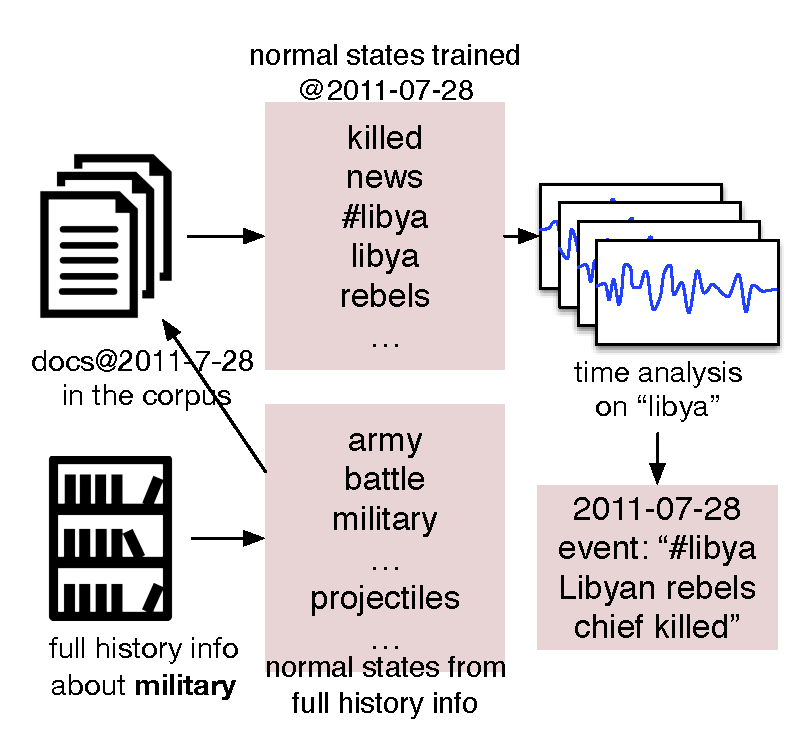
\includegraphics[height=7.0cm]{img/systemExample.pdf}
        }    
    \caption{Overview of how event detection systems use history information (left), and an example of our \textsc{FullReader} system process flow on how to detect the military related events (right).}
    \label{fig:modelDesc}
\end{figure*}

For example, in ideal conditions an event detection system for anti-terrorism has the knowledge about the normal state such as “the words ISIS and Syria are both high-frequent, while the word Russia is not so frequent as them”. 
With the knowledge of normal state, the system for anti-terrorism can detect the event of “Russia's anti-ISIS op in Syria” as Russia appeared more frequent than the normal state and appeared with ISIS and Syria. 
After detection, the ideal event detection system also updates the normal state by considering the new coming data.



\section{Related Works}
Although \cite{Wurzer:2015wq} points out that UMass\cite{Allan:2000wu} and its variants\cite{Petrovic:2010uj}\cite{petrovic2012using}\cite{Wurzer:2015wq} are the state-of-art systems on the Event Detection task for the newswire data, these systems still suffers from the lack of accuracy to applied on more general cyberspace data, such as tweets, emails, and reddit posts. 
The underlying reason is that the normalized Topic Weighted Minimum Cost metric (\(C_{min}\)) used in the Event Detection keep balance between miss and false alarm, which cannot work well on the .
Usually these traditional systems set the ratio of cost between miss alarm and false alarm to 10, preferring recall to precision on detecting events.

Study of event detection on text stream can be divided into three ways: word frequency based, text similarity based and topic model based.

Several word frequency methods have been developed for event detection such as Discrete Fourier Transform\cite{he2007analyzingDFT}, wavelet analysis \cite{weng2011eventWavelet}.
They treat the word's document frequency along timeline as time series and do the analysis in frequency domain. 
DFT method suffers the problem that it can not locate the time point for bursty.
Wavelet analysis based method's complexity is very high, so its scalability is limited. 

 Text similarity based online event detection methods\cite{petrovic2010streaming}\cite{mccreadiescalable}  suffer from the lexical variation which means different words describe the same events.
 Similarity based method can successfully detect the tweet which is retweeted by many times, but fails to find out the event which is described from many different perspectives.
 As a result, many events are duplicately detected due to their popularities, which may bury other events and overwhelm users with duplicated unwanted content.


In contrast, topic model can handle the lexical variation problem with word co-occurrence\cite{blei2003latent}.
%After \cite{blei2006dynamic} and \cite{wang2006topics} introducing time factor into topic model, a number of temporal model has been developed to different tasks.
As many events are highly related to topics, a number of methods based on topic model have been proposed for event detection, including online detection and offline detection.
Lau\cite{lau2012line} introduces an online topic model to track emerging events in microblogs.
It can deal with a massive of tweets, but it doesn't filter out the tweets related to user interests.
Diao\cite{timeUserLDA2012finding}\cite{diao2013unified} show that event detection can benefit from filtering out user interest related tweets. 
And Yan\cite{Yan:2015wm} models the bursty topic by incorporating burstiness of biterms as prior knowledge.
But they are different from ours.
As these models need the whole dataset as the input, they are offline detections, which is not scalability for large dynamic dataset such as micorblogs.
Instead, we gather user's self-description and the followings' self-description as user profile which is stable to characterize user interests. 
Based on this fine-grained user modeling information, user's long term interest related tweets and short term bursty event related tweets can be distinguished in online style, and can be efficiently applied on microblogs.

Since user modeling has the significant impact on users' activities on microblogs, the usage of user modeling has drawn attention in many research fields. 
\cite{zhao2013inferring} exploits user modeling information and network topology to infer user's role in social network.
\cite{yoshida2013toward} also introduces user modeling to community detection where some edges are not observable, but user profile can provide additional information.
Different from the above work, we do not only treat the user modeling result as an additional feature, but also an important representative factor for users, who are the source of information in microblogs.

User modeling can be carried out to obtain web users' demographics information \cite{culotta2015predicting} (e.g., gender, age, ethnicity, education, income, etc.).
Compared with demographics information, user interests' modeling can be verified more easily \cite{faralli2015large}. 

  尽管文献[1]指出UMass[2] 是FSD任务中最为精确的方法,但由于在Event Detection任务中,the metric used in this method单纯的使用normalized topic weighted minimum cost并不能准确的反映出它能够很好的说明网络空间中的事件检测的准确性。其原因在于计算公式中缩小了CFa的值(一般默认的方法将miss与false alarm的cost的比值设置为10:1),因而传统的方法倾向于扩大召回率而牺牲了准确率。这样的做法在处理newswire信息时并没有太大不妥,原因在于newswire中检测出的novel story是事件的概率极大。而一般的网络空间中不仅仅包含新闻,而且覆盖了各方面的信息【参见Twevent中对twitter信息覆盖面的文献】。在此种情况下,即便是novelty story,也不一定代表了事件(具体的例子见Section实验部分)。进一步的,我们认为UMass在应用到一般的网络空间的事件检测的准确率不高的原因是UMass没有对网络空间的正常状态进行有效的训练。UMass[2],LSH方法[3],k-terms Hashing[1]使用聚类簇来表示cyberspace的正常状态,然而对于twitter这种覆盖面极广的社交媒体,聚类簇的方法总是不能穷尽所有正常状态。【这里的说法不是很强健】
  与UMass,LSH,kterms等在向量空间或者在此基础上的哈希值进行聚类的方法不同,timeUserLDA[4]以及BBTM[5]对网络空间中的正常状态使用topic model进行刻画,将网络空间中的topics试图按照normal topics和bursty topics进行区分。该方法能够有效的检测到被人们广泛关注的bursty topics,这些bursty topics往往是我们需要我们检测的events的一部分。然而此类方法也有明显的缺陷,由于topic model使用对称的先验,因此其topic的规模倾向于相近的大小。然而人们在同一时间内对事件的关注度有限,事件受关注的程度也是趋向于power law分布的。这样,一些较小规模的事件不能被正确的检测出。因此,此类方法的特点是准确率高,但召回率低。进一步的究其本质,是timeUserLDA、BBTM等方法没有能够准确的训练网络空间的正常状态,较小的bursty event会被吸收进正常状态中。
另一类方法是以EDCoW[6]为代表的对词频的正常状态进行训练的工作,判断the degree of burstiness of terms,然而cyberspace中常用词频率变化并不明显,因此由这类词构成的事件往往并不容易被检测到,这一结果也由[7]证实。
与我们的工作最为相近的是Twevent[7],Twevent采用三个阶段的方式进行:tweet segment, event segment detection, event segment clustering。
Twevent 抽取tweet segment依赖于词典因而往往不能发现。。。
正常状态训练部分的相关工作。
Tedas[8], ESA[9], AIDR[10] 
TwitterMonitor[11], EDCoW[6], TwitInfo[12], Twevent[7], Leadline[13], TwiCal[14], ESA[9], Redites[15] 

Twitter Trending Topic Classification
%\begin{figure}
%    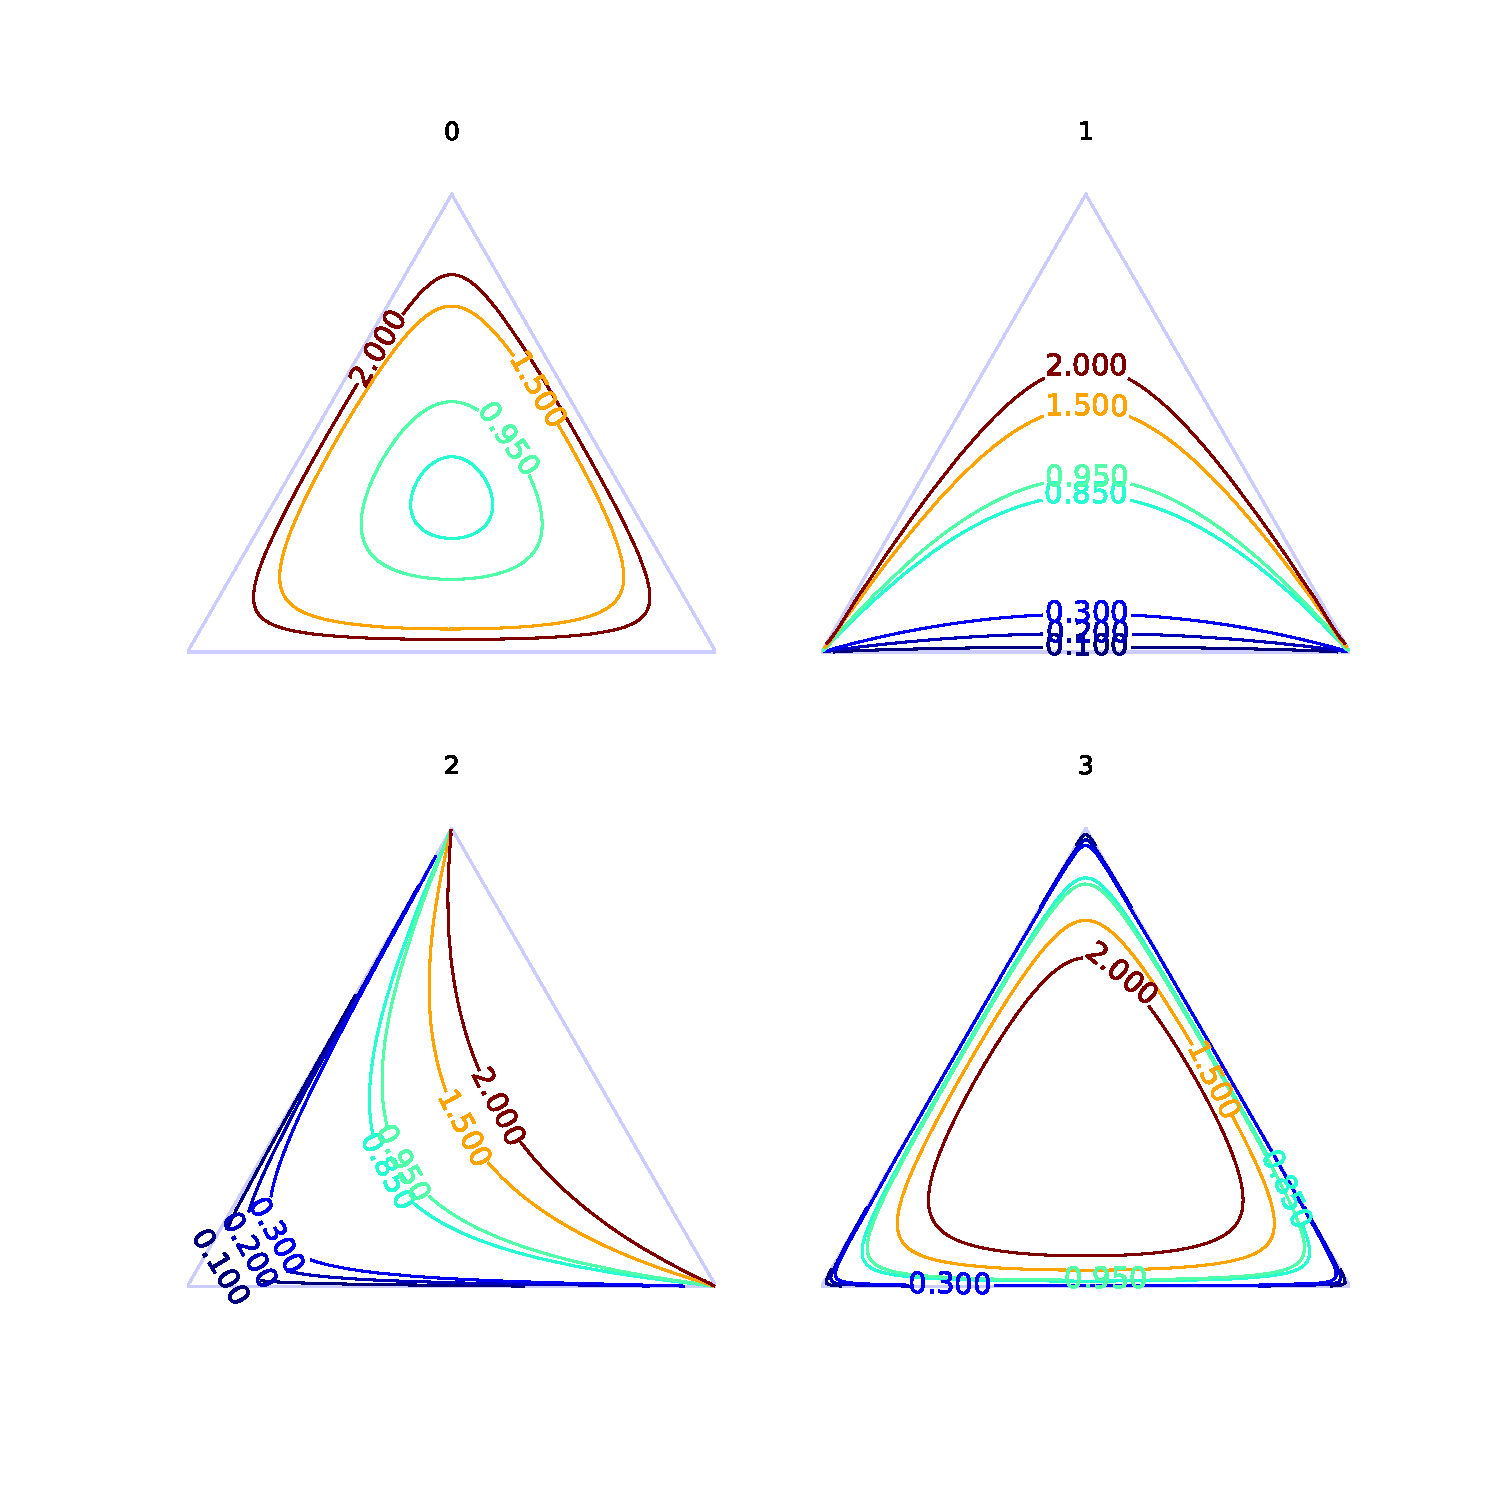
\includegraphics[height=7.7cm]{img/mlab_dirichlet_alpha_effects.pdf}
%\end{figure}
We use PageRank-HITS\cite{Yan:2015wq} algorithm to update score of categories in wikipedia.

%3*4 figures
\begin{figure*}[ht]
        \centering
        \label{fig:subfig} %% label for entire figure
        \subfigure[\(\alpha=(0.25,0.25,0.25)\)]{
                \label{fig:subfig:a} %% label for first subfigure
                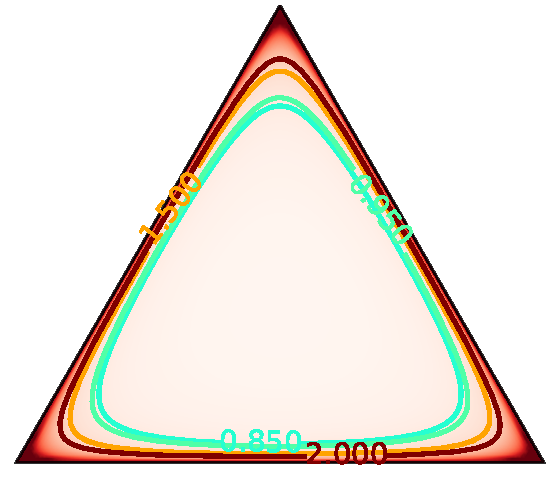
\includegraphics[height=3.21cm]{img/croppedDirichletGraph0.pdf}
        }
        \subfigure[\(\alpha=(0.5,0.5,0.5)\)]{
                \label{fig:subfig:b} %% label for second subfigure
                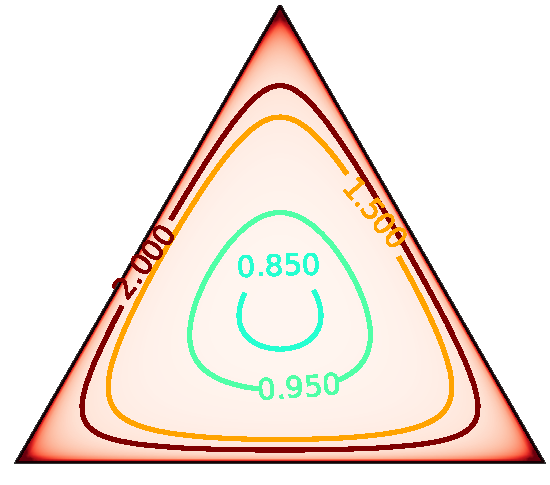
\includegraphics[height=3.21cm]{img/croppedDirichletGraph1.pdf}
        } 
        \subfigure[\(\alpha=(1.5,1.5,1.5)\)]{
                \label{fig:subfig:c} %% label for third subfigure
                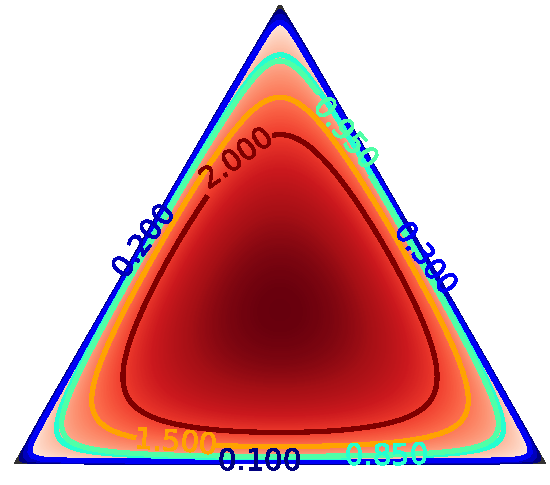
\includegraphics[height=3.21cm]{img/croppedDirichletGraph2.pdf}
        }
        \subfigure[\(\alpha=(2.5,2.5,2.5)\)]{
                \label{fig:subfig:a} %% label for first subfigure
                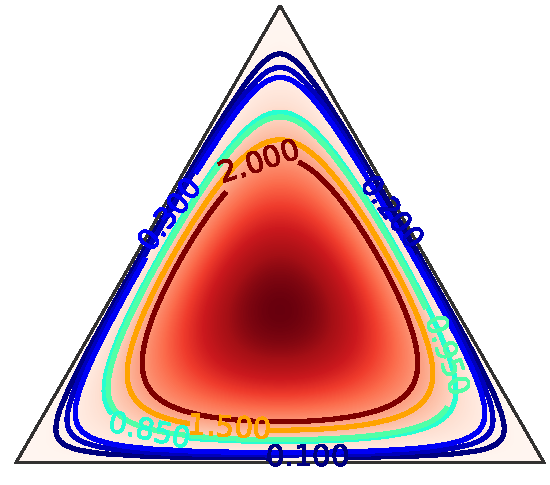
\includegraphics[height=3.21cm]{img/croppedDirichletGraph3.pdf}
        }\hspace{1in}
        \subfigure[\(\alpha=(0.25,0.25,0.75)\)]{
                \label{fig:subfig:d} %% label for third subfigure
                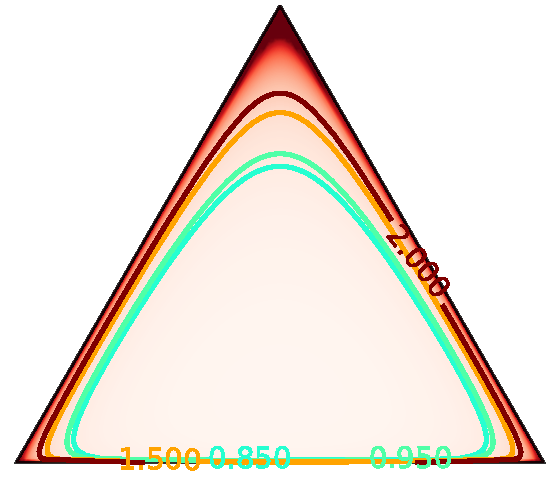
\includegraphics[height=3.21cm]{img/croppedDirichletGraph4.pdf}
        }
        \subfigure[\(\alpha=(0.5,0.5,1.5)\)]{
                \label{fig:subfig:d} %% label for third subfigure
                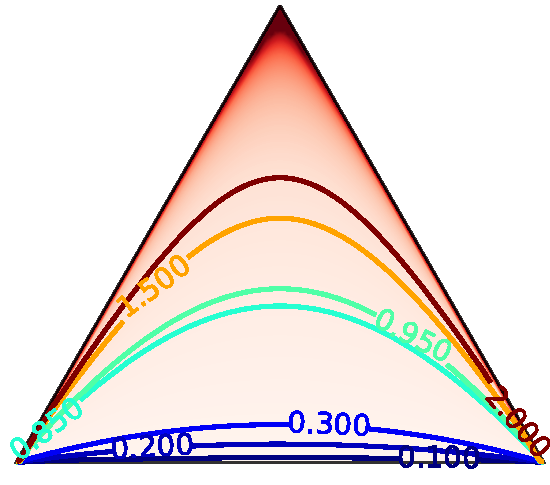
\includegraphics[height=3.21cm]{img/croppedDirichletGraph5.pdf}
        }
        \subfigure[\(\alpha=(1.5,1.5,2.5)\)]{
                \label{fig:subfig:d} %% label for third subfigure
                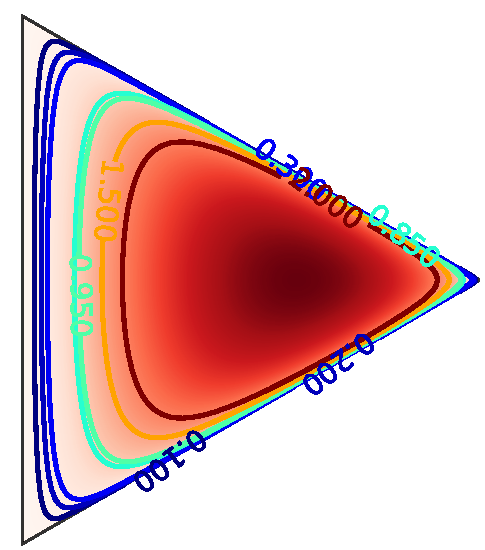
\includegraphics[height=3.21cm]{img/croppedDirichletGraph6.pdf}
        }
        \subfigure[\(\alpha=(2.5,2.5,3.5)\)]{
                \label{fig:subfig:a} %% label for first subfigure
                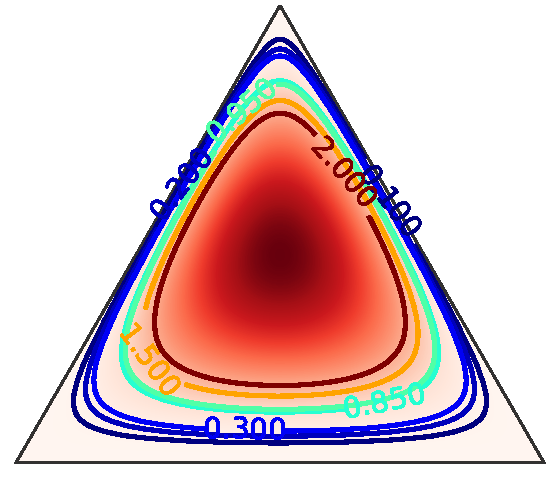
\includegraphics[height=3.21cm]{img/croppedDirichletGraph7.pdf}
        }\hspace{1in}
        \subfigure[\(\alpha=(0.25,0.75,0.75)\)]{
                \label{fig:subfig:d} %% label for third subfigure
                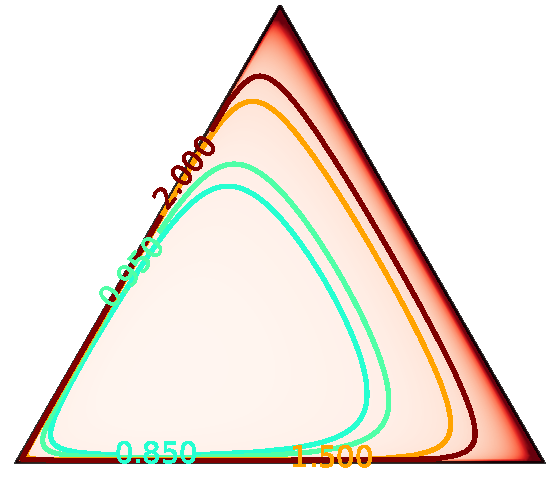
\includegraphics[height=3.21cm]{img/croppedDirichletGraph8.pdf}
        }
        \subfigure[\(\alpha=(0.5,1.5,1.5)\)]{
                \label{fig:subfig:d} %% label for third subfigure
                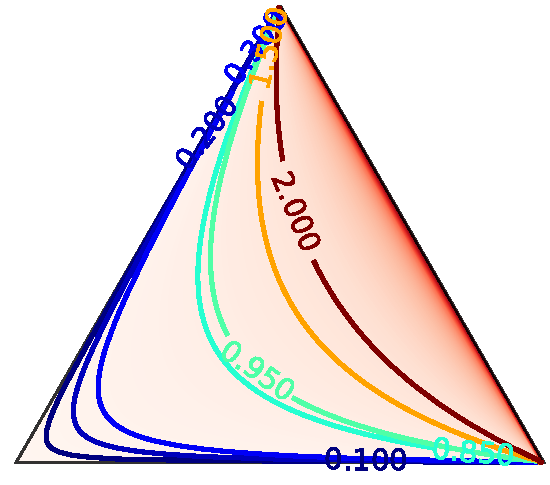
\includegraphics[height=3.21cm]{img/croppedDirichletGraph9.pdf}
        }
        \subfigure[\(\alpha=(1.5,2.5,2.5)\)]{
                \label{fig:subfig:d} %% label for third subfigure
                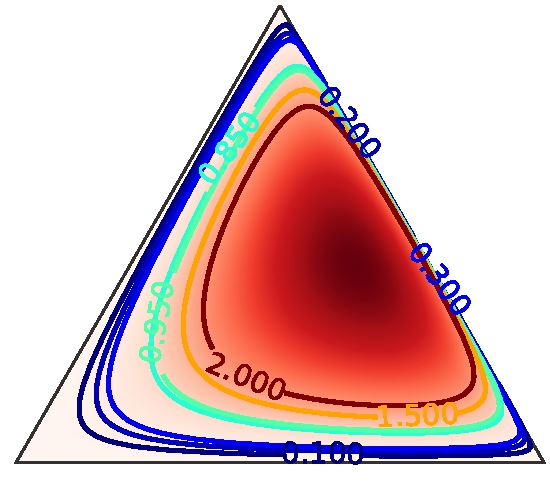
\includegraphics[height=3.21cm]{img/croppedDirichletGraph10.pdf}
        }
        \subfigure[\(\alpha=(2.5,3.5,3.5)\)]{
                \label{fig:subfig:a} %% label for first subfigure
                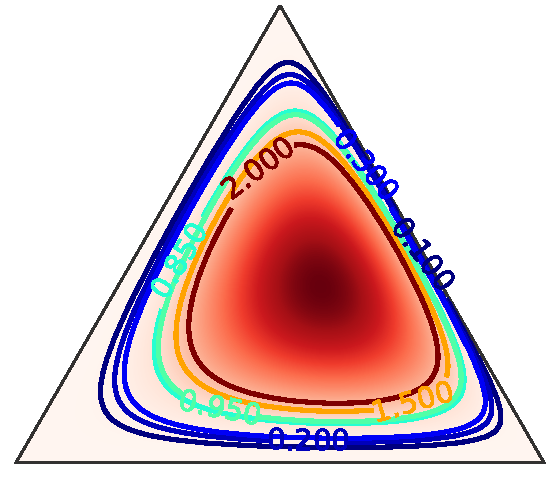
\includegraphics[height=3.21cm]{img/croppedDirichletGraph11.pdf}
        }
        \caption{Illustration of Drichlet distribution's probabilistic density on the 3-dimensional simplex when given different priors. (a-d) (e-h) (i-l)}
\end{figure*}



\section{Method}
\textbf{User profile.} User usually describes herself or himself by a piece of short text on microblog platform.
This short text can be a continuous string or an array of hash tags, e.g., "\textit{Co-founder of Twitter, Medium, and now Co-founder and CEO of Askjelly.com}" of Biz Stone or "\textit{\#Cloud}, \textit{\#YARN}" of @hadoopchina.
Though it's easy to estimate Biz Stone's interests by his self-description text, it's not always capable of doing so because some users' are very short.
To overcome this limitation, we define \textbf{user profile} \(\bm{p_u}\) as combining user \(u\)'s self-description text with the texts provided by \(u\)'s followings. 
Taking Biz Stone as an example, he follows 696 accounts, in which there are 60 founders, 27 CEOs, 21 Google related, and 9 medium related accounts, etc. 
This example demonstrates that user profile \(p_u\) can be augmented by gathering the followings' information.

\textbf{User modeling.} 
User modeling is used to capturing user's long term interests. 
For each user profile token, .
For example, Biz Stone's long term interests can be inferred as \textit{Social Media}, \textit{Business}, and \textit{Technology} from his user profile \textit{Medium}, \textit{CEO}, and \textit{Google} respectively.

The notations used in this paper are summarized in Table \ref{symbolsInModel}.
We consider \(u\)'s user timeline as  the triple \(\{uid, \bm{p_u},\bm{w_u}\} \), where \(\bm{p_u}\) represents user \(u\)'s profile and \(\bm{w_u}=\{(tweetid, t_{ud},w_{ud})\}\) means the set of tweets posted by user \(u\).
The element of \(\bm{w_u}\) is a triple of tweet id, time stamp \(t_{ud}\) and tweet content \(\bm{w_{ud}}\).



\textbf{Event.} We define the event in the given time window \(t\) as the set of tweets denoted by \( \{ \bm{w_{te}}\}\).
The event related tweets in set \( \{ \bm{w_{te}}\}\)  hold two properties: (1) it is different from user \(u\)'s long term interests and (2) it is similar with other tweets in the set.
The task of event detection is to find out all the events in corpus.
Different methods treat the above properties in different ways: LSH based methods\cite{petrovic2010streaming} treat the difference and simliarity in word vector space; while the topic model based methods\cite{timeUserLDA2012finding} take the semantic meaning into consideration.
Under the framework of topic model, we divide the topics into user interest related topics and bursty event related topics, and further promote an online learning model UMIETM.
\subsection{Normal States' Initialization}
%TODO
\begin{figure}
    \centering
    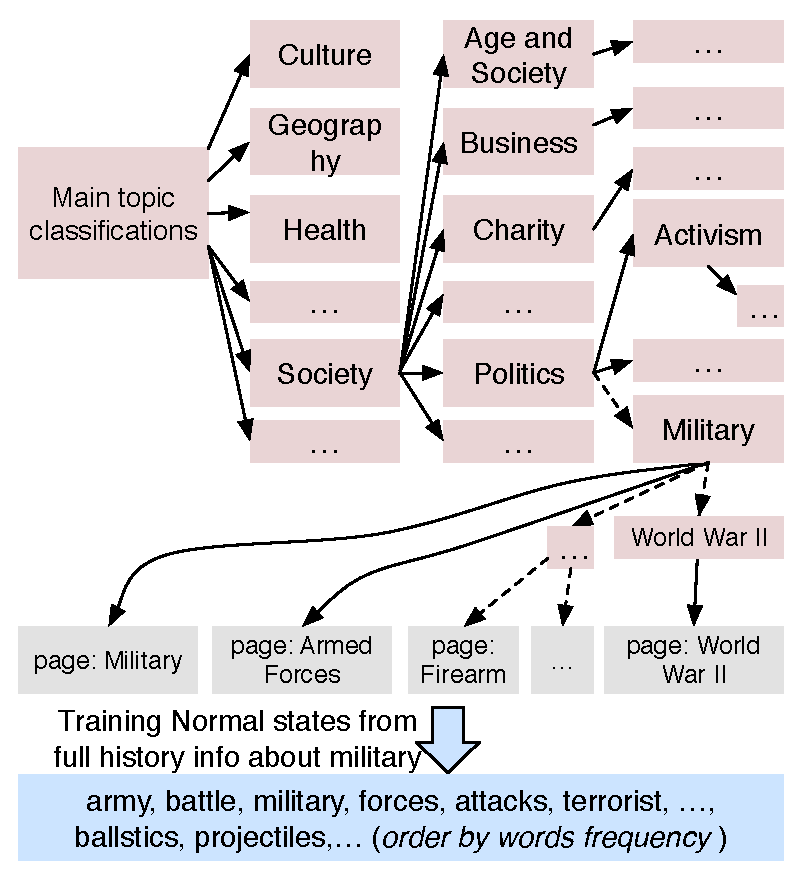
\includegraphics[width=1.0\columnwidth]{img/normalStatesFromHistoryInfo.pdf}  
    \caption{Illustration on how to train normal states from wikipedia,( an approximation to the full history information).}
    \label{fig:modelDesc}
\end{figure}

\textbf{HITS step.}
After the above step, we obtain PageRank scores for either queries or candidate replies. To propagate such information to the other side in the query-reply bipartite graph, we perform another random walk with links between queries and replies representing the structural information of hubs and authorities. %To incorporate prior information (obtained in the PageRank step) of queries and replies, we adopt a HITS variant in \citeauthor{deng2009generalized}~\shortcite{deng2009generalized}, called Co-HITS.



Formally, the bipartite graph $G=(V,E)$ has vertexes  $V=\{V_q \cup V_r\}$, where $V_q$ are queries and $V_r$ are replies. We define the weight matrix by a relevance scoring function $\phi(q,r)$ between queries and replies. $\phi(\cdot,\cdot)$ was learned via a \textit{learning-to-rank} model similar to ~\shortcite{burges2005learning} with rich features including textual similarity, translation models, as well as {\tt word2vec} word embeddings \cite{mikolov2013distributed}. In other words, $\phi(\cdot,\cdot)$ returns the relatedness between a query and a reply in the range $(0,1)$.

Moreover, since we would like to make use of PageRank scores for queries or replies, the HITS links are judged by not only the static relevance score $\phi(\cdot,\cdot)$, but also the information given by PageRank. To be concrete, the (unnormalized) weight matrix is given by either
\begin{equation}
\text{\quad \quad\quad\quad\!}\tilde{\mathbf W}_{ij} = \phi(q_i, r_j)\cdot q_i\quad\quad\quad\text{(query$\rightarrow$reply)}
\label{eqn:w1}
\end{equation}
\begin{equation}
\text{or\quad\quad\quad} \tilde{\mathbf W}_{ij} = \phi(r_i, q_j)\cdot {r}_i\quad\quad\quad\text{(reply$\rightarrow$query)}
\label{eqn:w2}
\end{equation}
Here, $q_i$ and $r_i$ are the \textit{i}-th element in the vectors $\mathbf q$ and $\mathbf r$, which are obtained in the PageRank phase by Equations~\ref{eqn:pagerank1}--\ref{eqn:pagerank2}. If information is propagated from queries to replies, we use the former equation for weight update, and \textit{vice versa}.


The mutual-reinforcing relationship of hub and authority scores can be expressed in matrix representation as follows.
\begin{align}
\mathbf{x}^{(i+1)} &= \alpha_x\cdot \big[\tilde{\mathbf W}\big]\,\mathbf{y}^{(i)}+(1-\alpha_x)\cdot \hat{\mathbf{x}}\label{eqn:HITS2}\\
\mathbf{y}^{(i+1)} &= \alpha_y\cdot \left[\big[\tilde{\mathbf W}\big]^\top\right]\mathbf{x}^{(i)}+(1-\alpha_y)\cdot\hat{\mathbf{y}} \label{eqn:HITS1}
\end{align}
where $\mathbf x$ is query scores, $\mathbf y$ reply scores; superscripts denote the number of local iterations in HITS update.
Each column of the weights is normalized to be a valid probability. Moreover, to compute the weight for $\mathbf{y}$, the matrix $\mathbf{\tilde W}^\top$ should be first row-normalized (given by $[\mathbf{\tilde W}]^\top$); otherwise, the effect of the prior $q_i$ in Equation~\ref{eqn:w1} is ruled out by column normalization.
Notice that the transition matrix is fixed in one step of HITS, but they may also change as our algorithm proceeds like the PageRank step. 

\subsection{Normal States' Maintenance}
Asymmetric-Prior-LDA
\begin{figure}[t]
    \centering
    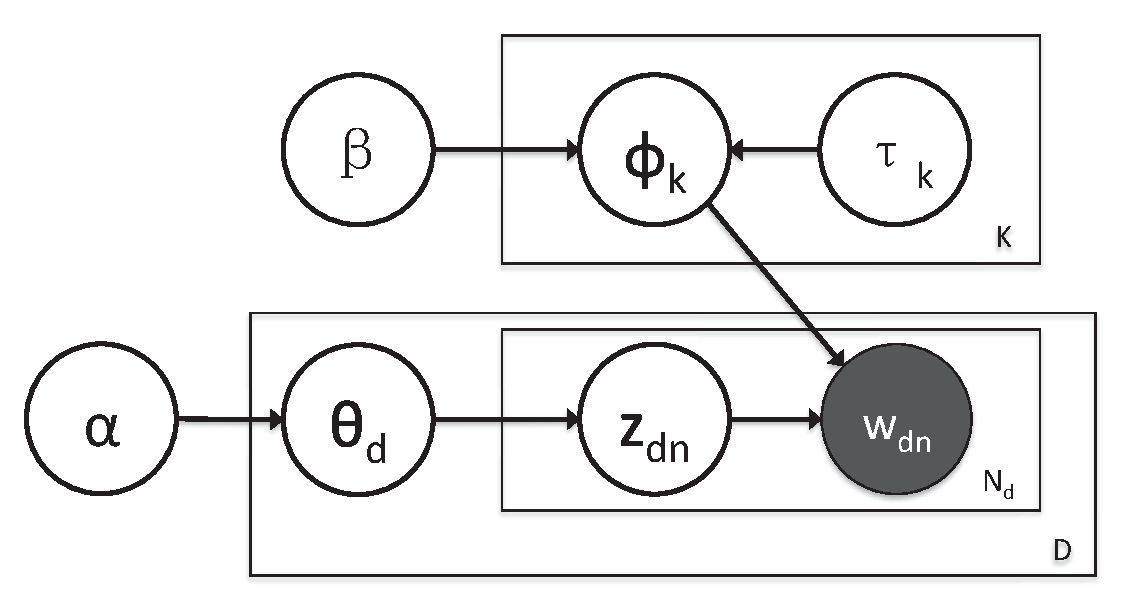
\includegraphics[height=3.5cm]{img/NTS.eps}
    \caption{Probabilistic model for training normal states by using history information.}
    %The convolution neural network for extracting character-level representations of words. Dashed arrows indicate a dropout layer applied before character embeddings are input to CNN.}
    \label{fig:cnn}
\end{figure}

\ \ Our theme modeling, want to learn the first \(k\) topics with Wikipedia Article \(k\) topics as close as possible, and we will be Wikipedia article \(k\) before 1000 words) was added to the theme of the word frequency word in the subject a priori distribution on the.
Learning to be the first \(k\) Subject polynomial distribution of the word, referred to as \(\phi_k \), Wikipedia article \(k \) distribution of topics for \(\tau_k \), then this formalized process is expressed as: \(\ phi_k \sim Dir(\beta + \tau_k) \).
Formal presentation of the explanation is: With prior knowledge \(\tau_k \) after the theme \(\phi_k \) is no longer simply rely on symmetric priori \(\beta \), different words right is not the same weight , such as a discussion of "fashion" theme in Wikipedia, it will refer to "dress", "grand", "blue", "gold" and other words, with the asymmetric priori \(\beta + \tau_k \) after in microblogging "fashion" theme "dress" the proportion will be increased in this way so that microblogging corpus theme tends to Wikipedia topic.
\(\tau_k \) in the first \(v \) words such as formula (\ref{eq: wikiPrior}).
Where \(S_k \) as a set of candidate words: high-quality information to use Wikipedia, we extract the theme \(phi_k \ \) in the higher-word word frequency candidate set \(S_k \).
We can control set \(S_k \) in size, the size of the control is usually set for 1000.
The number of frequency \(n_{kv} \) for the word \(v \) (\ k) appears in the Wikipedia article themes of: (\ref{wikiPrior eq}).
If the word \(v \) does not appear in the candidate set \(S_k \), and then set a priori knowledge \(\tau_{kv} = 0 \), otherwise, the word frequency is proportional to \(n_{kv} \) with the prior knowledge of weight \(W\).
In the latter experiment, we will be on a priori knowledge of weights \(W \) will be discussed.

\begin{enumerate}[noitemsep]
    \item for each topic \(k \in \{1,\cdots,K\}\),
    \begin{enumerate}
        \item word distribution on the topic \(\phi_k \sim Dirichlet(\beta+\tau_k)\).
    \end{enumerate}
    \item for each document \(d \in D\),
    \begin{enumerate}
        \item topic distribution on the document \(\theta_d \sim Dir(\alpha)\)
        \item for each word index \(n \in \{1,\cdots,N_d\}\),
        \begin{enumerate}
            \item word's topic assignment \(z_{dn} \sim Multinomial(\theta_d)\),
            \item word \(w_{dn} \sim Multinomial(\phi_{z_{dn}})\)
        \end{enumerate}
    \end{enumerate}
\end{enumerate}

\begin{equation}
\label{eq:wikiPrior}
\begin{aligned}
\tau_{kv}=
\left\{ \begin{aligned}
W \frac{n_{kv}}{\sum_{v\in S_{kv}}n_{kv}} &,v\in S_{k} \\
0&,v \notin S_{k}\\
\end{aligned}\right.
\end{aligned}
\end{equation}

\begin{equation}
\label{eq:LDAgibbs}
\begin{aligned}
&p(z_{dn}=k|w_{dn}=v,z_{\neg{dn}},w_{\neg{dn}},\alpha,\beta,\tau)\\
&\ \ \propto \frac{n_{dk}+\alpha}{n_{d,.}+K\alpha}\frac{n_{kv}+\tau_{kv}+\beta}{n_{k,.}+\tau_{k,.}+V\beta}
\end{aligned}
\end{equation}

\begin{algorithm}[H]
    \caption{UPIETM batch learning algorithm} %title
    \label{alg:UPIETMbatch} %label
    \begin{algorithmic}[1] %this 1 means the showing of line number in algorithm
    \STATE initiate the topic label and the statistics
    \FOR {\(i=1:I_1\)}
        \FOR{\(u\) in  user set U}
            \FOR{\(n\) = \(1:P_u\)}
                \STATE sample profile's hidden topic \(s_{un}\) by (\ref{timeUserTagLDAIVsamplingForS})
                \STATE update \(s_{un}\), \(c^{(p)}_{u,k}\) and \(c^{(p)}_{k,v}\)
            \ENDFOR%end of n
        \ENDFOR%end of u
    \ENDFOR%end of i
    \FOR{iteration \(i=1:I_2\)}
        \FOR{\(t=1:T\)}
            \FOR{\(u\) in  user set \(U_t\)}
                \FOR{\(d\) = \(1: D_u\) }
                    \STATE{sample \(y_{ud}\) and \(z_{ud}\) by (\ref{timeUserTagLDAIVJointSamplingForY0Z}), (\ref{timeUserTagLDAIVJointSamplingForY1Z}) }
                    \IF{\(y_{ud}=0\)}
                        \STATE{update \(z_{ud}\), \(y_{ud}\), \(c^{(0)}_u\), \(c^{(0)}_{u,k}\), \(c^{(0)}_{k,v}\)}
                    \ELSE
                        \STATE{update \(z_{ud}\), \(y_{ud}\), \(c^{(1)}_u\), \(c^{(1)}_{t,k}\), \(c^{(1)}_{t,k,v}\)}
                    \ENDIF
                    \FOR{\(n\) in \(1,\cdots,N_{ud}\)}
                        \STATE{sample \(x_{udn}\) by (\ref{timeUserTagLDAIVsamplingX0}), (\ref{timeUserTagLDAIVsamplingX1}})
                        \IF{\(x_{udn}=0\)}
                            \STATE{update \(x_{udn}\), \(M^{\rho}_0\), \(c^{(B)}_v\)}
                        \ELSE
                            \STATE{update \(x_{udn}\), \(M^{\rho}_1\), \(c^{(0)}_{k,v}\), \(c^{(1)}_{t,k,v}\) }
                        \ENDIF
                    \ENDFOR%end of n
                \ENDFOR%end of d
            \ENDFOR%end of u
        \ENDFOR%end of t
    \ENDFOR%end of i
    \end{algorithmic}
\end{algorithm}


\subsection{Detecting Events from Normal States}
The state of attention of social issue k at time t in cyberspace is binary, namely at the peak or not at the peak. We denote it by hidden binary variable sk,t, which is 1 or 0. We do the inference for the hidden variable sk,t according to Poisson distribution according to Reference10,11. If the state of attention of social issue k at time t is "not at peak", then the probability density function is 
\(p([Ax_(k,t) ]|s_(k,t)=0)=e^(-μ_0 )  μ_0^([Ax_(k,t)])/([Ax_(k,t)]!)\) otherwise the probability density function is \(p([Ax_(k,t) ]|s_(k,t)=1)=e^(-μ_1 )  μ_1^([Ax_(k,t)])/([Ax_(k,t)])\)
In the above functions the symbol \(x_{k,t}\) denotes the attention of social issue k at time t , the symbol A denotes the constant, \(μ_0\) and \(μ_1\) represent the average of \([Ax_(k,t)]\) at peak and not at peak respectively. The state sk,t is inferred from \(ratio=p([Ax_(k,t) ]|s_(k,t)=0)/p([Ax_(k,t) ]|s_(k,t)=1) \).
In calculation, we use the log ratio to determine whether the attention is at peak as in equation (1). logratio>0 indicates that the attention of social issue k at time t is not at peak, otherwise at peak. As the attention xk,t is often between 0.01% and 5% in our experiment, we set the constant A in log ratio equation to be〖10〗^4。
	\(logratio=-(μ_0-μ_1 )+[Ax_(k,t)](log⁡μ_0 -log⁡μ_1)\)
After the data preprocessing, we get the air pollution state sequence\((a_t)_(t=1,…T)\) and the attention state sequence of each social issue \((s_(k,t))_(t=1,…,T;k=1…n)\), where T denotes the number of time windows.

\begin{algorithm}
\caption{Spectral Clustering Based Event Phrase Extraction}
\label{alg:eventKeywordsSearchMethod}
\KwIn{\(\mathcal{B}_{k,t},\mathcal{G}_{k,t},\tau\)}
\KwOut{\(\mathcal{C}_{k,t}\)}
\(n_{k,t}\)=number of connected component in \(\mathcal{G}_{k,t}\)\\
\For{\(n \in \{ n_{k,t}, \cdots, |\mathcal{G}_{k,t}|\}\) }{
    \(\mathcal{C}_{k,t}=SpectralClustering(\mathcal{G}_{k,t},n)\)\\
    \If{\(min_{i\in \{1,\cdots,n\}} Density(\mathcal{C}_{k,t,i},\mathcal{G}_{k,t})>\tau\)}{
        return \(\mathcal{C}_{k,t}\)
    }
}
\end{algorithm}


\begin{figure}
\centering
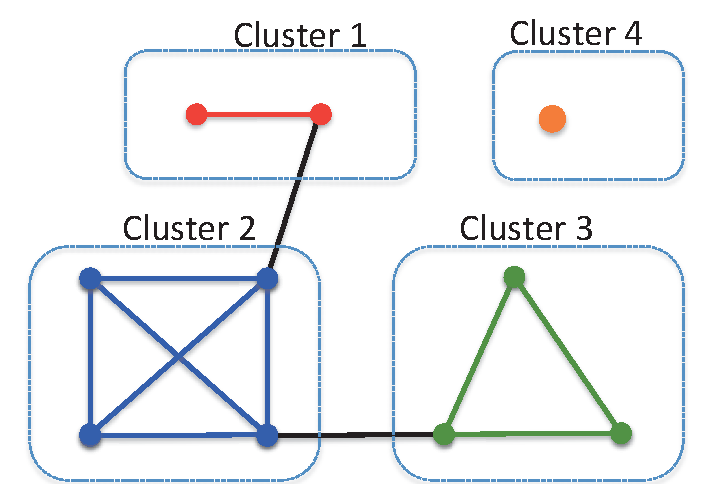
\includegraphics[height=3cm]{img/wordClusterGraph.eps}
%todo
\caption{Hot words between the heat pattern forming word time window edge weight calculated by the PMI obtained between words, to obtain spectral clustering clustering clustering}
\label{fig: windowsBurstyWordGraph}
\end{figure}

\textbf{event} phrase Mining
% Refer to bursty.py
\ \ Microblogging mining events can be represented by a variety of ways, a single word, phrase, or topic.
Here we use the form of phrase, said event.
In this paper, the phrase indicates that the event is due to the fact that: the same period of time when there are multiple areas of internal hot words appear, a collection of hot words \(\mathcal{B}_{k, t} \) between the hot words great probability is interrelated. For example, observed "mac", "os", "lion" three words are in a state of emergency.
In fact, the state of emergency three words is to publish a new system "mac os lion" event caused by Apple, in order to find the association between words and events, we use spectral clustering based search methods.

As shown in Figure \ref{fig: windowsBurstyWordGraph} below, we will one area, a hot word of the time window and hot words between to diagram.
Hot words set \(\ mathcal {B}_{k, t} \) formed in FIG using \textbf{hot word graph} \(\mathcal {G}_{k, t} = (\mathcal{B}_{k, t}, \mathcal{E}_{k, t}) \) indicates,
\(\mathcal{E}_{k, t} = \{(a, b) | a \in \mathcal{B}_{k, t}, b \in \mathcal {B} _ {k, t }, PMI (\mathcal{D}_{k, t}, a, b)> 0 \} \), where \(PMI (\mathcal{D}_{k, t}, a, b) \) the field \(k \) time window \(t \) related microblog \(\ mathcal {D} _ {k, t} \) on the word \(a \) and the word \(b \) point metric information between each other.
% Refer to bursty.py getSimGraph () function

Given a field \(k \) and the time window \(t \), in which the number of events can not be determined in advance.
The two most extreme situations are: events coarse granularity, said the event is equal to the number of Figure \(\ mathcal {G} _ {k, t} \) in the number of connected components; events finer granularity display, event number equal to \(\ mathcal {G} _ {k, t} \) the number of points.
To do this, we use the Density to the degree of density of quantum graphs \(2 \#Edge / (\# Node \ cdot (\# Node-1)) \), the more the greater if the edge density in the range of Density in \((0,1] \).
Density can be a good indicator to determine the size indicates the event: too many unrelated phrases to put together an event can not be represented, too fine particle size, such as a single word can represent only part of the event; only in close co-occurrence of the phrase to a reasonable It indicates that the event granularity.
To this end, we have designed events phrase search algorithm \ ref {alg: eventKeywordsSearchMethod}: We try to find a reasonable number of spectral clustering Clustering \(n \), let \(n \) from a smaller value ( event corresponds to coarser granularity representation) to start the search, then the most likely cluster cluster size is too large, its performance is the clustering results in one or more small Density indicators; continue to increase the number of clusters \(n \), the event represents reduced size, reduced the size of clusters of clusters, thus making the Density index increases; when all cluster clustering Density indicators are larger than the threshold \(\tau \), the search terminates, returning clustering results \(\mathcal{C}_{k, t}\).
As the above process algorithm \ref{alg: eventKeywordsSearchMethod} description line 2 to line 5, we use in practice \(\tau = 0.6 \).
We call \(\mathcal{C}_{k, t} \) results in each cluster to cluster \textbf{event} phrase.

\textbf{detected events related to micro-blog}
\ \
By algorithm \ref{alg:eventKeywordsSearchMethod} find art \(k \) time window \ \(t \) within the \(| \mathcal{C}_{k, t} | \) events phrase later, you can also further find each event and the corresponding event phrase microblogging.
We looked at the first \(i \) events phrase \(\mathcal{C}_{k, t, i} \),
The phrase based on the number of elements distinguish the event, there are three situations: (1) the phrase event more than two hot words, he said while the event is not a phrase between any two words We have a very strong relationship between the co-occurrence, so just pay attention to the co-occurrence relationship stronger side; (2) event phrase has two hot words; (3) the event is only a hot word in the phrase.
Weibo text length is shorter, not all of the microblogging event will include the phrase \(\mathcal{C}_{k, t, i} \) in all the words.
Such as those on "Apple released the new system mac os lion" event, the event phrase "mac", "os", "lion" does not need to appear in all of the micro-Bo, just check the co-occurrence of a strong relationship between the two words appear together whether in an article in the field \(k \) time window \(t \) micro-Bo: If there is, then added to the events related to the collection \(\ mathcal {D} _ {k, t, i} \) in.
For the case of a third cluster cluster contains only a hot word, we only need to identify areas \(k \) contains the hot word of all micro-blog, and add the event to the relevant set \(\ mathcal{D }_{k, t, i} \) in.
Ultimately, we can get the field \(k \) next time window \(t \) in the event the phrase relating to events microblogging \(\{(\mathcal{C}_{k, t, i}, \mathcal{D}_{k, t, i}) \}_{i=1}^{| \mathcal{C}_{k, t} |} \).

\section{Experiments}
\begin{figure}
        \centering
        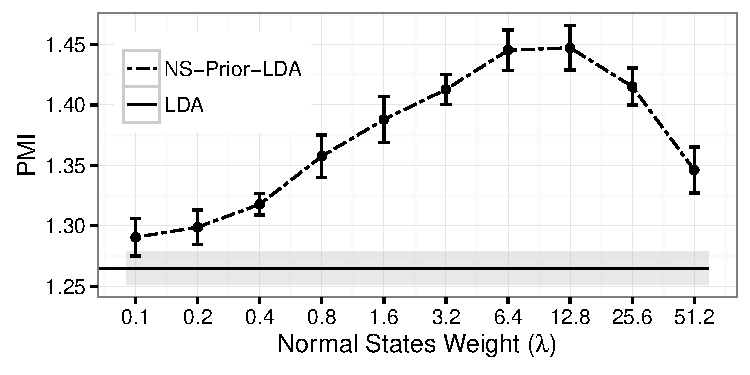
\includegraphics[height=4.0cm]{img/pmi.pdf}
        \caption{History State Portion}
\end{figure}
\begin{table}
\centering
\caption{Normal State Training Performance}
\label{my-label}
\scalebox{0.8}{
    \begin{tabular}{|l|l|l|}
    \hline
    Model & History State & PMI \\ \hline
    LDA & None  & 1.265 \(\pm\) 0.013     \\ \hline
    BBTM\cite{Yan:2015wm} & None    & 1.467 \(\pm\) 0.017     \\ \hline
    NST\(^{(-)}\)   &   \begin{tabular}[c]{@{}l@{}}\footnotesize{Learned by LDA}\\ \footnotesize{from Wikipedia}\end{tabular} & 1.439 \(\pm\) 0.010     \\ \hline
    NST         & \begin{tabular}[c]{@{}l@{}}\footnotesize{Derived from Categories} \\\footnotesize{of Wikipedia}\end{tabular} & 1.523 \(\pm\) 0.017     \\ \hline
    \end{tabular}
}
\end{table}

\begin{table*}[ht]
\centering
\caption{My caption}
\label{my-label}
\begin{tabular}{|cc|cc|cc|cc|}
\hline
\multicolumn{2}{|c|}{\textit{Security}} & \multicolumn{2}{c|}{\textit{Vehicles}} & \multicolumn{2}{c|}{\textit{Health}} & \multicolumn{2}{c|}{\textit{Sport}} \\ 
\begin{tabular}[c]{@{}c@{}}History\\ State\end{tabular} & \begin{tabular}[c]{@{}c@{}}Normal\\ State\end{tabular} & \begin{tabular}[c]{@{}c@{}}History \\ State\end{tabular} & \begin{tabular}[c]{@{}c@{}}Normal \\ State\end{tabular} & \begin{tabular}[c]{@{}c@{}}History \\ State\end{tabular} & \begin{tabular}[c]{@{}c@{}}Normal \\ State\end{tabular} & \begin{tabular}[c]{@{}c@{}}History \\ State\end{tabular} & \begin{tabular}[c]{@{}c@{}}Normal \\ State\end{tabular} \\ \hline
Army & killed & aircraft & air & medical & weight & league & season \\ 
Battle & news & train & plane & patients & loss & season & win \\ 
military & \#libya & airport & flight & treatment & diet & club & team \\ 
Forces & libya & station & time & disease & pain & cup & deal \\ 
attacks & rebels & flight & ship & health & cancer & football & year \\ 
terrorist & people & pilot & news & brain & health & game & sign \\ 
troops & police & aviation & boat & cancer & lose & games & jagr \\ 
Killed & war & gear & airport & patient & tips & round & richards \\ 
soldiers & libyan & passenger & force & blood & treatment & championship & cup \\ 
commander & attack & drive & fly & body & fat & player & time \\ 
Front & u.s. & navigation & hurricane & clinical & hair & match & arsenal \\ 
Units & gaddafi & departure & navy & care & skin & division & fans \\ 
captured & army & takeoff & coast & surgery & body & win & nasri \\ 
campaign & forces & aviator & home & research & healthy & goals & city \\ 
fighting & pakistan & navigator & crash & type & surgery & teams & league \\ 
siege & afghanistan & runaway & irene & syndrome & blood & play & players \\ 
officers & military & departure & train & system & brain & stadium & player \\ 
guards & attacks & airbus & sea & medicine & acne & coach & signed \\ 
allied & troops & miles & aircraft & eye & diabetes & players & contract \\ 
lieutenant & dead & landing & jet & physician & eye & record & run \\ \hline
\end{tabular}
\end{table*}


\begin{table*}[ht]
\centering
\caption{My caption}
\label{my-label}
\begin{tabular}{|l|l|l|l|l|}
\hline
Method & \begin{tabular}[c]{@{}l@{}}Recall@ \\ Benchmark1\end{tabular} & \begin{tabular}[c]{@{}l@{}}Precision@ \\ Benchmark2\end{tabular} & \begin{tabular}[c]{@{}l@{}}Recall@ \\ Benchmark2\end{tabular} & \begin{tabular}[c]{@{}l@{}}DERate(Duplicate \\ Event Rate)\end{tabular} \\ \hline
UMass System & 0.882 & 0.138 & 0.941 & 0. 071 \\ \hline
LSH & 0.824 & 0.095 & 0.803 & 0.302 \\ \hline
TimeUserLDA & 0.353 & 0.536 & 0.071 & 0.054 \\ \hline
Twevent & 0.824 & 0.697 & 0.641 & 0.113 \\ \hline
EDCoW & 0.412 & 0.756 & 0.119 & 0.290 \\ \hline
BBTM & 0.647 & 0.809 & 0.170 & 0.045 \\ \hline
Our Method & 1.000 & 0.894 & 0.950 & 0.042 \\ \hline
\end{tabular}
\end{table*}

\begin{table}[]
\centering
\caption{Twitter data set description}
\label{my-label}
\begin{tabular}{|l|r|}
\hline
Time range & \begin{tabular}[c]{@{}r@{}}2011/06/30\\ -2011/09/15\end{tabular} \\ \hline
Tweet number & 36,627,434 \\ \hline
Event number in Benchmark1 & 17 \\ \hline
Event number in Benchmark2 & 523 \\ \hline
\end{tabular}
\end{table}
% \begin{table}[]
% \centering
% \caption{My caption}
% \label{my-label}
% \begin{tabular}{|l|l|l|l|}
% \hline
% \multicolumn{1}{|c|}{\begin{tabular}[c]{@{}c@{}}Time \\ range\end{tabular}} & \multicolumn{1}{c|}{\begin{tabular}[c]{@{}c@{}}Tweet \\ number\end{tabular}} & \multicolumn{1}{c|}{\begin{tabular}[c]{@{}c@{}}Event number \\ in Benchmark1\end{tabular}} & \multicolumn{1}{c|}{\begin{tabular}[c]{@{}c@{}}Event number \\ in Benchmark2\end{tabular}} \\ \hline
% \begin{tabular}[c]{@{}l@{}}2011/06/30-\\ 2011/09/15\end{tabular} & 36,627,434 & 17 & 523 \\ \hline
% \end{tabular}
% \end{table}

\begin{table*}[ht]
\centering
\caption{Events about \textit{vehicles} detected by systems between 2011-07-20 and 2011-07-30}
\label{my-label}
\begin{tabular}{|l|L{3cm}|l|c|}
\hline
\multicolumn{1}{|c|}{Date} & \multicolumn{1}{c|}{Event key words} & \multicolumn{1}{c|}{Representative event tweet} & \multicolumn{1}{c|}{\begin{tabular}[c]{@{}c@{}}Number of \\ event tweet\end{tabular}} \\ \hline
7/20/11 & \begin{tabular}[c]{@{}l@{}}American, Airlines, \\ order, planes\end{tabular} & \begin{tabular}[c]{@{}l@{}}NDTV: American Airlines orders 460 new planes from \\ Boeing, Airbus http://bit.ly/p1ZgYG\end{tabular} & 31 \\ \hline
7/23/11 & \begin{tabular}[c]{@{}l@{}}China, bullet, train, \\ collision\end{tabular} & \begin{tabular}[c]{@{}l@{}}China Bullet Train Collision: 33 Dead, 190 Injured \\ http://huff.to/qEq6Yx\end{tabular} & 67 \\ \hline
7/26/11 & \begin{tabular}[c]{@{}l@{}}Morocco, military, \\ plane, crash\end{tabular} & \begin{tabular}[c]{@{}l@{}}BBC News - Morocco military plane crash kills 78 \\ http://t.co/uwnLv8L\end{tabular} & 36 \\ \hline
7/27/11 & Air, Canada & \begin{tabular}[c]{@{}l@{}}Smoke in galley forces Air Canada flight back to airport. \\ Plane landed safely in Sydney, Australia after dumping fuel\end{tabular} & 48 \\ \hline
7/30/11 & \begin{tabular}[c]{@{}l@{}}Caribbean, Airlines, \\ crashes, Guyana\end{tabular} & \begin{tabular}[c]{@{}l@{}}Caribbean Airlines Jet Crash-Lands In Guyana All 163 \\ Passengers, Crew Survive http://t.co/qPVD3WJ\end{tabular} & 57 \\ \hline
\end{tabular}
\end{table*}

\begin{table*}[ht]
\centering
\caption{My caption}
\label{my-label}
\begin{tabular}{|l|L{3cm}|l|l|}
\hline
Date & Event key words & Representative event tweet & \begin{tabular}[c]{@{}l@{}}Number of \\ event tweet\end{tabular} \\ \hline
7/20/11 & \begin{tabular}[c]{@{}l@{}}Serbia, crimes, \\ fugitive, arrests\end{tabular} & Serbia: Serbia arrests last war crimes fugitive-TV- Reuters & 27 \\ \hline
7/20/11 & Somalia, famine & \begin{tabular}[c]{@{}l@{}}UN declares famine in Somalia. What can we do to save \\ 3.7million lives? http://bit.ly/r1Rq7R\end{tabular} & 89 \\ \hline
7/21/11 & \begin{tabular}[c]{@{}l@{}}U.S., military, \\accept, gay, \\lesbian, openly\end{tabular} & \begin{tabular}[c]{@{}l@{}}RT @cnnbrk: Pentagon is set to certify that the U.S. military \\ is prepared to accept openly gay and lesbian service members \\ \#dadt\end{tabular} & 20 \\ \hline
7/22/11 & \begin{tabular}[c]{@{}l@{}}Norway, Oslo,\\ attacks, bombing\end{tabular} & \begin{tabular}[c]{@{}l@{}}Terror Attacks Devastate Norway: A bomb ripped through \\ government offices in Oslo and a gunman...˙http://dlvr.it/cLbk8\end{tabular} & 557 \\ \hline
7/23/11 & Gunman, rink & \begin{tabular}[c]{@{}l@{}}Gunman Kills Self, 5 Others at Texas Roller Rink \\ http://dlvr.it/cLcTH\end{tabular} & 43 \\ \hline
7/26/11 & \begin{tabular}[c]{@{}l@{}}Kandahar, mayor, \\ suicide, attack\end{tabular} & \begin{tabular}[c]{@{}l@{}}TELEGRAPH{]}: Kandahar mayor killed by Afghan suicide \\ bomber: The mayor of Kandahar, the biggest city in south \_\end{tabular} & 25 \\ \hline
7/28/11 & Ft., Hood, attack & Possible Ft. Hood Attack Thwarted http://t.co/BSJ33hk & 20 \\ \hline
7/28/11 & \begin{tabular}[c]{@{}l@{}}Libyan, rebel, \\ gunned\end{tabular} & \begin{tabular}[c]{@{}l@{}}Libyan rebel chief gunned down in Benghazi \\ http://sns.mx/prfvy1\end{tabular} & 44 \\ \hline
\end{tabular}
\end{table*}

\begin{figure*}
    \label{fig:algorithm}
    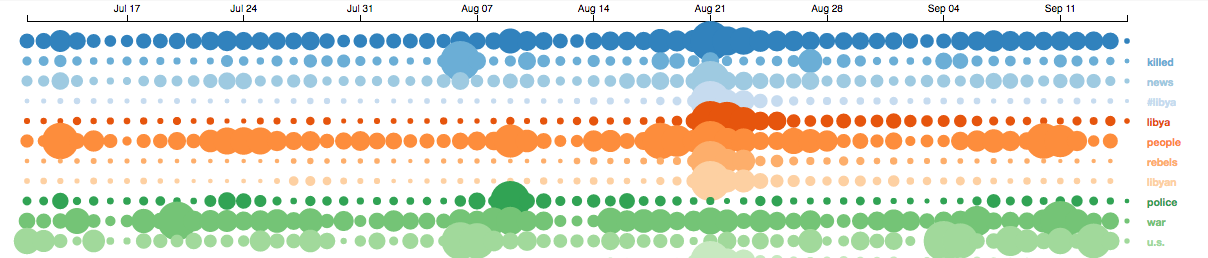
\includegraphics[width=1.0\textwidth]{img/screenShot.png}
\end{figure*}

\subsection{Data set}
Dataset
We conduct the empirical analysis on a twitter dataset which is constructed by \cite{petrovic2012using} and widely used by previous event detection researches \cite{petrovic2013can} \cite{Wurzer:2015wq}. 
Due to the developer policy of Twitter\footnote{https://dev.twitter.com/overview/terms/policy}, \cite{petrovic2012using} only redistributes tweets' IDs\footnote{http://demeter.inf.ed.ac.uk/cross/docs/fsd\_corpus.tar.gz}.
We collect the tweets' contents according to the IDs with the help of Twitter API. 
The dataset contains 36,627,434 tweets which spans from 2011/06/30 to 2011/09/15.

Here we present the effectiveness of our proposed algorithm UMIETM and the efficiency of its online performance.
We evaluate the efficiency by perplexity, precision for event detection. 
We check the time cost and complete likelihood for efficiency.
% We are going to design the experiment to show the effectiveness of distinguishing user interests and events.
% Firstly, user profile can help to model user interests.
% In this experiment we compare to the baseline of user interest modeling\cite{sun2013serendipity}.
% Secondly, event detection can be enhanced by filtering out user interests.
%\subsection{Experiment Settings}
%We demonstrate our method can work very well on real dataset.

Weibo is a popular Chinese microblogging service\footnote{http://en.wikipedia.org/wiki/Sina\_Weibo/}.
We crawl weibo data by  its public API\footnote{http://open.weibo.com/} from Jan 2012 to Dec 2012.
To improve the quality of analyzing on tweets, we do necessary pre-processing: (1) splitting dataset by week, (2) segmenting Chinese words, (3) removing stop words and low frequency words whose document frequency in its time window is less than 3, (4) removing tweets whose token number is less than 3.
To model user interests better,  we remove users from dataset who has less than 2 hashtags in profile.
After pre-processing we get 252 thousand users, 16 million tweets and 251 million tweet tokens listed in Table \ref{statisticsOfDataset}.

We compare our model UMIETM with twitterLDA, timeUserLDA, Author-LDA, and our model's variant IETM.
Author-LDA combines the tweets posted by same author into a single document, then run standard LDA on the assembled tweets.
TwitterLDA is designed for topic modeling on twitter.
We compare with Author-LDA and TwitterLDA for confirming the significance of distinguishing user interests from events in microblog.
TimeUserLDA is designed for retrospective event detection in microblog, and considers to distinguish events from user interests.
We compare with timeUserLDA to show the impact of user profile.
The variant IETM (\textit{Interest and Event Topic Model}) models user's interests and events without the help of user profiles.
%UMIETM benifits from modeling user profiles.

%To demonstrate the necessary of user profiles, we compare it to its variant IETM (Interest and Event Topic Model) which only consider the tweets shown in figure \ref{fig:IETM}.
%IETM also run in online learning way.

We set the asymmetric \(\alpha\) and symmetric \(\beta=0.01\) for UMIETM, where \(\alpha\) will be optimized by Gibbs EM algorithm\cite{wallach2008structured}.
\(\alpha=0.1\), \(\beta=0.01\) are set for all remaining models. 
After cross validation we find that UMIETM and IETM perform best on \(K=90\) and \(E=30\), \(\kappa=0.01\).
To compare equally, we set the same topic number for Author-LDA, twitterLDA, timeUserLDA (which means when we run models offline on 1 time window, we shall set 120 topics for all, and 150 topics on 2 time windows and so on).

To verify the role of user profiles played, we set UMIETM(-) as the degradation of UMIETM, which take symmetric prior \(\alpha\).

In this subsection, we illustrate the performance of UMIETM in which user profile is considered.

\textbf{Quantitative Measure.}
We initialize UMIETM and IETM by batch learning on data from first week to third week, then run them in online learning way from fourth week to ninth week.
On each week we calculate their perplexities\cite{wallach2009evaluation}, where \(perplexity(D_{test})=\exp{\{-\frac{\sum_{u=1}^{U}\sum_{d=1}^{D_u}\log{p(w_{ud})}}{\sum_{u=1}^{U}\sum_{d=1}^{D_u}N_{ud}}\}}\) and \(p(w_{ud})=(1-\pi_u)\sum_{k=1}^{K}\theta_{uk}\prod_{n=1}^{N_{ud}}(\phi_{s,w_{udn}}(1-\rho)+\phi_{k,w_{udn}}\rho)+\pi_u \sum_{k=1}^{K}\eta_{t,k}\prod_{n=1}^{N_{ud}}(\phi_{s,w_{udn}}(1-\rho)+\phi_{k,w_{udn}}\rho)\).
The others are trained from first week to third week, and the held out perplexities are calculated on data from fourth week to ninth week.
TimeUserLDA and IETM's perplexities are smaller than User-LDA, twitterLDA as they both consider distinguishing user interests from events.

In Table \ref{tab:heldoutPerplexity} the perplexity of UMIETM is 3107.8, and much smaller than others. It demonstrates that user profile is significant for tweet stream's modeling.

In Table \ref{tab:metrics}, we evaluate the events detected by models. We asked the annotators to label the event with score 1, and non-event related topic as 0. 
The precision and recall is illustrated, where UMIETM(-) performs slightly better than IETM. 
And UMIETM outperforms UMIETM(-) in detecting high quality event. 
A reasonable analysis is that UMIETM uses the profile information sufficiently by asymmetric priors. 
In this way, we also prove that the well exploiting of user profile information is important to model user interests and events on tweets. 
%\subsubsection{Precision of Event Detection}

\textbf{Case Study} 
Some events detected by our UMIETM model are shown in Table \ref{fig:event}.
Comparing with UMIETM, timeUserLDA fails to discover the \textit{shoddy construction} event in the second week, while IETM reports this event as \textit{bi, women, elegant, adoption, engineering, reed}. Obviously IETM fails to distinguish this event from user interests.
UMIETM filters users' interests like \textit{bi, women, elegant, adoption} using their profile {\#baby, \#women}, and detect the event.
\subsection{Efficiency}
We implement our methods on mallet\footnote{http://mallet.cs.umass.edu/dist/mallet-2.0.7.tar.gz}, and run them on Linux server with 8 cores(2.00GHz) and 64GB memory.
In this subsection, we verify the convergence and online performance of our online learning algorithm. 

\textbf{Convergence.}
The convergence of algorithm is vital in real time streaming environment. 
UMIETM needs several Gibbs sweeps to find out the optimal parameters of model.
But the size of data is usually large even spitted into time windows.
The time complexity of UMIETM is \(O(I_1K|P|+I_2K|W|+I_2E|W|)\) given in section \ref{subsec:online}.
It suggests that the more iterations Gibbs sampling have to do, the less efficiently our model performs. 
Fortunately UMIETM is very economic to its stable state and does not need so much iterations.
As suggested by \cite{wallach2009rethinking} and \cite{jian2014factorOfTopicModel}, we choose LDA with asymmetric priors as baseline, which is much more comparable than standard LDA on microblog dataset.
We run UMIETM on the first three time windows. 
Correspondingly we only use the tweets in these time windows for LDA with asymmetric priors.
Burn-in period is set to 20 and optimize interval also 20, which means the priors are optimized every 20 iterations as the red curve in Fig \ref{fig:completeLoglikelihood}.

One of the criteria for stopping Gibbs sampling is that the complete log likelihood is stabilized.
We stop UMIETM after 50 iterations since the complete log likelihood only increases 0.02\% in last iteration.
It will take LDA(asymmetric priors) 300 minutes to run 1000 iterations, and 20 minutes per 10 iterations for UMIETM.
There is a trade-off between the effectiveness by more iterations and efficiency by less,  we set the iteration number as 10 in online setting.
After 10 iterations the UMIETM's complete log likelihood will increase no more than 0.2\%.
% \subsubsection{Soundness}
% As the online learning for UMIETM is an approximated version of batch learning for UMIETM, the soundness should be confirmed before applying it in the real enviroment.
%[todo] We also want to show that online learning for UMIETM does not  sacrifice the accuracy. 
%Comapring the held out perplexity.

\textbf{Online Performance.}
%Figure \ref{fig:completeLoglikelihood} shows that the log likelihood increases less than 0.1\% after 12 iterations.
%Our experiment shows UMIETM has good convergence that the complete log likelihood increases less than 0.15\% after 10 iterations.
As verified in the above subsection \textit{Convergence}, we run 10 Gibbs sweeps for each time window in online learning phase.
When UMIETM is implemented in online way, it doesn't have to revisit the tweets in previous windows. 
So its time cost in each window is proportional to the data size of current window  as shown in Figure \ref{fig:onlinelearningResult}.
In average, online UMIETM can process five thousand tokens per second.
%Memory cost grows slightly and the increased memory cost only depends on the size of vocabulary.

LSH based event detection on microblogs is used by \cite{petrovic2010streaming},\cite{mccreadiescalable}. 
The former one detects events as the cluster of tweets by LSH, and the latter one extends this method on distributed machines. 
They both only use the cosine similarity without considering semantic meaning of words. 
So LSH based method may split the same event into clusters of similar tweets.
However LSH based method reports 10578 events in 7th time window, and 10901 events in 8th window. 
The other problem of LSH based event detection method is that the bad design may lead unstable performance. 
The tweets are mapped into LSH defined space in a skew way which is illustrated in Fig \ref{fig:onlinelearningResult}.
The other comparison is timeUserLDA which is designed for retrospective event detction. 
The purple line in Fig \ref{fig:onlinelearningResult} goes up straightly as timeUserLDA has to revisit previous tweets to make a decision whether the tweet is event related. 
The perplexity of online UMIETM on the 11 time window in Fig \ref{fig:onlinelearningResult} is \(3036.44\pm397.14\). 
And the average precision of detecting high quality event is 0.22.
Both indicators demonstrate that UMIETM can perform well in online learning way. 
\subsection{Application on Reddit}

\section{Conclusions \& Future Work}
Microbiolog is mixed with user interests and external events.
The quality of event detection in microblog depends on how we distinguish them.
We exploit user profile to discover events by filtering out user interest-related tweets.
We further treat the arriving data as stream and run the detection in online learning style.
The experiments demonstrates that our method is effective and efficient for online event detection in microblogs.


%
% The following two commands are all you need in the
% initial runs of your .tex file to
% produce the bibliography for the citations in your paper.
\bibliographystyle{abbrv}
\bibliography{paperbib}  % sigproc.bib is the name of the Bibliography in this case
% You must have a proper ".bib" file
%  and remember to run:
% latex bibtex latex latex
% to resolve all references
%
% ACM needs 'a single self-contained file'!
%
%APPENDICES are optional
%\balancecolumns
\end{document}
